\documentclass[10pt,a4paper]{article}
\usepackage[margin=1.9cm]{geometry}
\usepackage{graphicx}
\usepackage{booktabs}
\usepackage{amsmath}

\setlength{\parindent}{0pt}

% more compact section headings (no extra package needed)
\makeatletter
\renewcommand\section{\@startsection{section}{1}{\z@}%
  {-1.6ex \@plus -.4ex \@minus -.2ex}{0.6ex}{\normalfont\large\bfseries}}
\makeatother
\setlength{\parskip}{4pt}

\title{Network Science HS26 -- Assignment\\[2pt]
\large Bioinformatics Network Investigation: an enzyme structural graph}
\author{Ermin Mumic}
\date{}

\begin{document}
\maketitle
\vspace{-1.5em}

\section{Data and approach}

The edge list has 220 rows; every edge is listed in both directions. Loaded as a simple
undirected graph, the network has $N = 51$ nodes (IDs 1--51), $L = 110$ links, no self-loops,
average degree $\langle k\rangle = 4.31$ and density $0.086$. All numbers are computed in the
accompanying notebook; [\S n] refers to its sections.

Every property is measured and then compared with null models, chosen by what they keep fixed:
\emph{ER networks} $G(N,L)$ keep only $N$ and $L$ (is the property more than a consequence of size
and density?); \emph{degree-preserving randomisation} by link swaps keeps every node's degree (is it
more than a consequence of the degrees?). Each comparison uses 1000 random networks with fixed seeds;
the p-value is the share of random networks at least as extreme as the real one, with the direction
of the test fixed in advance and significance level $\alpha = 0.05$. Mean $\pm$ standard deviation
of the random networks are reported. If no random network reaches the real value, we report
$p < 1/n$ (one-sided) or $p < 2/n$ (two-sided).

\section{Global structure and degrees}

The network is connected. Its average distance is $\langle d\rangle = 5.04$ and its diameter is 12;
node 25 is its centre (smallest eccentricity, 6) [\S1]. These distances are much longer than chance:
$\langle d\rangle = 2.80 \pm 0.05$ in ER networks (594 of 1000 connected and used) and
$2.80 \pm 0.03$ under degree-preserving randomisation; the diameters are $5.72 \pm 0.63$ and
$5.11 \pm 0.32$ ($p < 0.002$ and $p < 0.001$, one-sided). The long distances are therefore not
explained by size, density or degrees, but by how the nodes are wired. The drawing
(Figure~\ref{fig:communities}, left) shows an elongated network, which fits these measurements.

The degrees range only from 2 to 6; 23 of the 51 nodes (45\%) have degree 4 [\S2]. Compared with ER
networks, both the largest degree ($k_{\max} = 6$ vs $9.20 \pm 1.13$) and the spread of the degrees
($\sigma_k = 1.08$ vs $1.93 \pm 0.19$) are smaller (two-sided, $p < 0.002$ for both). The network has
no hubs and its degrees are \emph{more uniform} than random -- the opposite of the broad degree
distributions typical of many real networks.

\section{Local structure and degree correlations}

The clustering coefficient is $C = 0.238$: on average about a quarter of the pairs of a node's
neighbours are linked [\S3]. This is about 3--4 times the random value
($0.081 \pm 0.026$ for ER, $0.061 \pm 0.022$ degree-preserving, $p < 0.001$ for both), so the network
contains more triangles than its size, density or degrees produce. The degree assortativity is
$r = 0.169$ against $-0.025 \pm 0.090$ in degree-preserving randomisations (two-sided $p = 0.028$)
[\S4]. This is significant at $\alpha = 0.05$ but not at $0.01$; we treat it only as weak evidence
that linked nodes tend to have similar degrees.

\section{Important nodes}

Degree, closeness, betweenness and eigenvector centrality select different nodes; their Pearson
correlations range from 0.07 (betweenness--eigenvector) to 0.61 (closeness--betweenness) [\S5].
The five nodes with the highest betweenness (0.37--0.44, the next node has 0.19) are linked one
after another and form the \textbf{path 36--8--25--26--27}, with the centre node 25 in its middle.
Nodes 26, 27 and 36 have only degree 4: they are important because of their position, not their
number of links. Each lies on roughly 37--44\% of the shortest paths between
other nodes, so many shortest routes between parts of the network run along this path. Eigenvector
centrality instead selects a densely linked group of degree-6 nodes (20, 33, 35, 43, 47; 6 of 10
possible links).

\section{Communities}

\begin{figure}[t]
  \begin{minipage}[c]{0.46\textwidth}
    \centering
    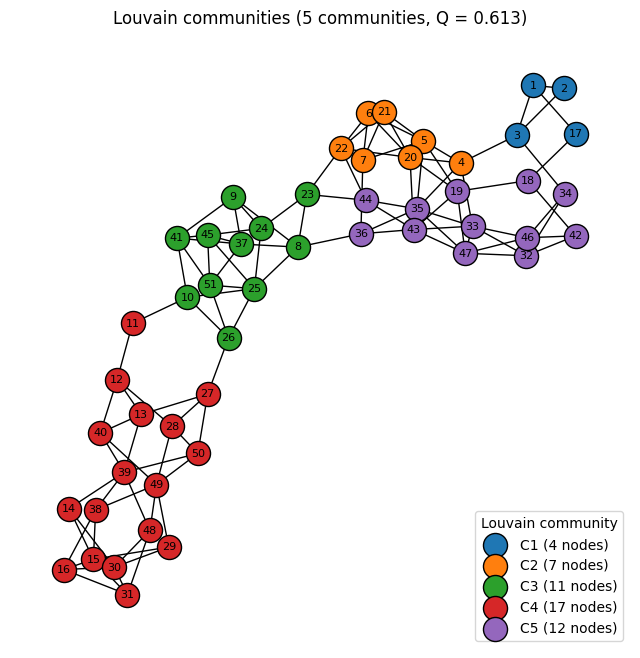
\includegraphics[width=0.9\linewidth]{figures/communities.png}
  \end{minipage}\hfill
  \begin{minipage}[c]{0.5\textwidth}
    \centering
    \begin{tabular}{lccc}
    \toprule
     & $\langle d\rangle$ & diam. & $C$ \\
    \midrule
    ER (mean of 1000) & 2.80 & 5.7 & 0.081 \\
    degree-preserving (mean) & 2.80 & 5.1 & 0.061 \\
    \textbf{enzyme network} & \textbf{5.04} & \textbf{12} & \textbf{0.238} \\
    ring lattice ($N = 51$, $k = 4$) & 6.76 & 13 & 0.500 \\
    \bottomrule
    \end{tabular}
  \end{minipage}
  \caption{Left: the network (Kamada--Kawai layout) coloured by the five Louvain communities.
  Right: average distance, diameter and clustering of the network compared with random networks
  and a ring lattice (\S7).}
  \label{fig:communities}
\end{figure}

Louvain (fixed seed) finds five communities with modularity $Q = 0.613$ (Figure~\ref{fig:communities}, left)
[\S6]. A search for high modularity also finds $Q > 0$ in random networks, so we repeated the search in
1000 degree-preserving randomisations: they reach only $Q = 0.409 \pm 0.019$ ($p < 0.001$). The
network therefore has stronger community structure than random networks with the same degrees.
The communities are cohesive (internal link density 0.25--0.67 vs 0.086 overall) and separated
(only 16 of 110 links, 15\%, run between communities).

All five are weak communities; none is
strong, because nodes 3, 17, 4, 23, 11, 36 and 44 have at least as many links outside their
community as inside.

To judge how convincing the partition is, we compared it with label propagation, edge betweenness
(Girvan--Newman) and Louvain with resolution $\gamma = 2$. C3 is found almost unchanged by all
three methods. The nodes of C4 stay together (except node 11), although two methods split C4 into
two or three smaller groups. The border between C2 and C5 is grouped differently by every method,
and the nodes that change community (e.g.\ 11, 17, 18, 23, 35, 36, 44) are largely the same boundary
nodes as above. The path of Section~4 runs from C5 (node 36) through C3 (8, 25, 26) into C4 (27).

\section{Random, small-world, scale-free or lattice-like?}

Following Lecture~4, we place the network between random networks and a ring lattice with the same
$N$ ($\kappa = 2$, $k = 4$; Figure~\ref{fig:communities}, right) [\S7].
The network is \emph{not random} (distances, degrees, clustering and communities all differ
significantly from random networks) and \emph{not scale-free} (degrees 2--6, no hubs). It is also
\emph{not small-world} in the sense of the lecture: its clustering is clearly above random, but its
distances are not ``almost as short as in a random network'' -- they are almost twice as long, and
the diameter is close to that of the lattice. It is \emph{partly lattice-like}: $\langle d\rangle$ lies
a bit more than halfway from random to lattice (0.57 of the way), $C$ about a third (0.37).

\section{Beyond the summary: a part held by two links}

The drawing suggested one end part joined to the rest by few links. Louvain found this part as C4
from the links alone, and the community table showed only two external links [\S8]. These are the
\textbf{links 10--11 and 26--27}; removing them splits the network into C4 (17 nodes) and the
remaining 34 nodes. A third of the network is thus reached only through two links, so every path
between C4 and the rest must use one of them. This feature is invisible in $\langle k\rangle$, the
degree distribution, $C$ or $\langle d\rangle$, which do not depend on where the links lie. It is
consistent with the long distances and with nodes 26 and 27 lying on the high-betweenness path.

\section{Conclusion and limitations}

The enzyme graph is an elongated network of nodes with very uniform degrees, made of locally dense
groups that are joined by few links: it is neither random, scale-free nor small-world, but has
lattice-like distances. Its main network-specific features are (i) the path 36--8--25--26--27 that
carries many shortest routes, (ii) community C4, attached to the rest only through the links 10--11
and 26--27, and (iii) boundary nodes such as 11, 23 and 36 whose community depends on the method.

\emph{Limitations.} Community detection algorithms are heuristics, and modularity maximisation can
merge small communities (resolution limit), so border nodes should not be over-interpreted. The
small-world property is defined by how $\langle d\rangle$ grows with $N$, which cannot be measured on
a single network; the ring lattice is only a reference (all degrees 4, $L = 102$). With many tests,
a single borderline result such as the assortativity ($p = 0.028$) may be a false alarm. Finally, we
have no information on what the nodes represent, so the structure is described but not explained
biologically.

\end{document}
